\documentclass[11pt]{article}
\usepackage[margin=1in]{geometry}
\usepackage{amsmath,amssymb}
\usepackage{graphicx}
\usepackage{booktabs}
\usepackage{float}
\usepackage{caption}
\usepackage{hyperref}
\usepackage{xcolor}
\graphicspath{{figures/}}
\captionsetup{font=small,labelfont=bf}
\hypersetup{colorlinks,linkcolor=blue!60!black,citecolor=blue!60!black,urlcolor=blue!60!black}

\newcommand{\Real}{\operatorname{Re}}
\newcommand{\Imag}{\operatorname{Im}}
\newcommand{\infbeyn}{InfBeyn}

\title{Spectrum transition through the sonic point:\\
are the tools ready?}
\author{Hunt Feng}
\date{\today}

\begin{document}
\maketitle

\begin{abstract}
The goal is to follow the spectrum of the magnetic-nozzle eigenvalue problem (thesis Eq.~3.6) as the throat
Mach number $v_m$ is moved through $1$. This note checks the two available tools against that goal.
(i) \infbeyn{} as used for the non-transonic flows works in principle for every $v_m\neq1$, but on the plain
Chebyshev grid its cost explodes as $v_m\to1$: the resolvent solutions develop a layer of width
$\sim|1-v_m|$ at the throat, the degree per solve grows like $100/|1-v_m|$, and the scan at $v_m=0.99$ does
not resolve with $N=4096$. A one-line change, a $\sinh$ map clustering the grid at the throat, removes the
problem: every case down to $|1-v_m|=10^{-4}$ resolves with $N\le1024$, and full certified scans take
seconds to a minute or two. (ii) The Frobenius idea (select the regular solution at the sonic throat) is
correct and is what makes the transonic problem well posed, but the thesis implementation is not accurate
enough: its series coefficient $c_2$ drops terms, the profile derivatives come from finite differences,
and the shooting search is not exhaustive. Re-solving the accelerating transonic flow with \infbeyn{} and the
regularity condition imposed as a collocation row confirms the first thesis eigenvalue to $10^{-4}$, corrects
the second by $0.07$, and shows that thesis modes 3--8 are not eigenvalues. (iii) The eigenvalues move at a
speed $|d\omega/dv_m|$ that grows as $v_m\to1$ while their spacing stays $O(1)$; a $v_m$ grid uniform in
$\ln|1-v_m|$ with step $\Delta v_m\approx0.1\,|1-v_m|$ (about 23 points per decade on each side) tracks
every mode in the window.
\end{abstract}

\section{Problem and what ``crossing the sonic point'' means}

The eigenvalue problem is (thesis Eq.~3.6)
\begin{equation}
  \begin{split}
  T(\omega)\tilde v \equiv{}&
  \omega^2 \tilde v + 2i\omega\left(v_0\tilde v' + v_0'\tilde v\right)
  + (1-v_0^2)\tilde v'' \\
  &- \Big(3v_0+\frac1{v_0}\Big)v_0'\tilde v'
  - \Big[\Big(1-\frac1{v_0^2}\Big)v_0'^2 + \Big(v_0+\frac1{v_0}\Big)v_0''\Big]\tilde v = 0
  \end{split}
  \label{eq:nep}
\end{equation}
on $z\in[-1,1]$ with fixed-open ($\tilde v(-1)=\tilde v'(1)=0$) or Dirichlet boundaries, and
\[
  v_0(z)=\big[-W_k\big(-(B/B_m)^2v_m^2e^{-v_m^2}\big)\big]^{1/2},
\]
with the same field as the non-transonic study ($B_0=1$, $R=1.5$, $\Delta=1/3$).

Figure~\ref{fig:profiles} shows the family. For $v_m<1$ the whole profile is subsonic ($k=0$) and for $v_m>1$
supersonic ($k=-1$). The two families meet at $v_m=1$ in a profile with a corner at the throat:
$1-v_0\approx 2.32|z|$ for $v_m\to1^-$, and $v_0-1\approx2.32|z|$ for $v_m\to1^+$. The smooth accelerating
transonic profile is a third branch through the same X-point; it is not the limit of either family.
Moving $v_m$ through $1$ therefore means passing through a singular limit, and on each side the coefficient
$1-v_0^2$ of $\tilde v''$ is of size $|1-v_m^2|$ in a throat layer of width $\sim|1-v_m|$
(Fig.~\ref{fig:profiles}, right).

\begin{figure}[H]
  \centering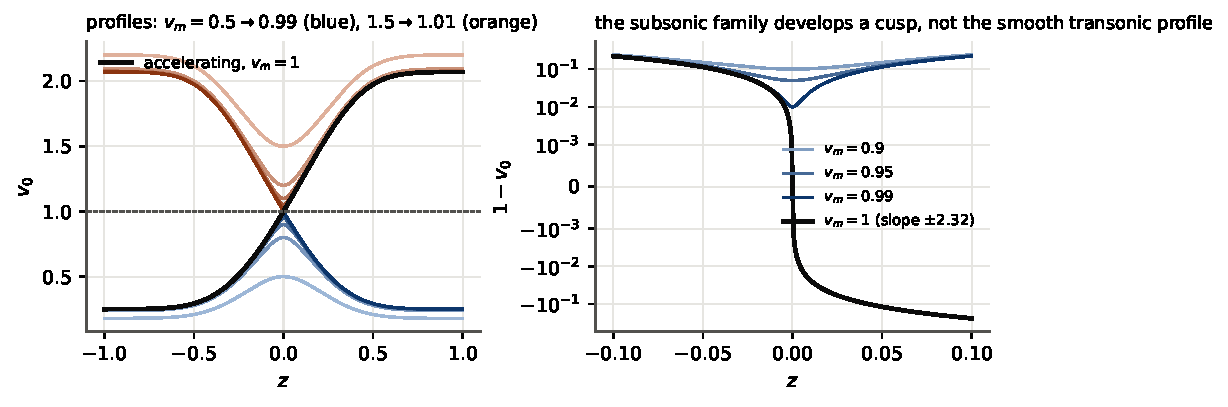
\includegraphics[width=\textwidth]{profiles_near_sonic}
  \caption{Left: profiles for $v_m=0.5,0.8,0.9,0.95,0.99$ (blue) and $1.5,1.2,1.1,1.05,1.01$ (orange), with the
  smooth accelerating transonic profile (black). Right: $1-v_0$ near the throat. The subsonic family
  approaches a cusp, while the transonic profile crosses $v_0=1$ with slope $2.32$.}
  \label{fig:profiles}
\end{figure}

\section{Is \infbeyn{} ready for $v_m\to1$?}

\paragraph{On the plain grid it is not.} Every resolvent solve $T(\omega)^{-1}V$ in a scan must resolve a
layer at the throat. There the equation is nearly singular, and solutions oscillate on a scale
$\sim(1-v_0)/|\omega|$. The adaptive Chebyshev solver doubles $N$ until the tail is below $10^{-12}$.
Figure~\ref{fig:res} (orange) shows the degree it reaches: $N=256$ at $v_m=0.5$, $1024$ at $0.9$, $2048$ at
$0.95$, and unresolved at $4096$ for $0.99$, close to $N\approx100/|1-v_m|$. The cost per dense solve grows
like $N^3$ and the memory like $N^2$ per worker. Table~\ref{tab:timing} shows the effect on a full scan of the
fixed-open window: $9$\,s at $v_m=0.5$ and $376$\,s at $v_m=0.9$, with five estimates left unpolished. The
$v_m=0.95$ scan ran for more than $40$ minutes and exhausted the $15$\,GB of the workstation (12 workers,
each factoring $4097\times4097$ complex matrices) before it was stopped. At $v_m=0.99$ no solve resolves at
all. Extrapolating, a plain-grid sweep to $|1-v_m|=10^{-2}$ is a cluster job, and $10^{-3}$ is out of reach.

\paragraph{With a throat-clustered grid it is.} Replacing $x\in[-1,1]$ by $z=\sinh(Lx)/\sinh L$, which
compresses the grid at the throat by $L/\sinh L$, with
\begin{equation}
  L = 1 + 1.5\ln\frac1{|1-v_m|}\qquad(|1-v_m|<0.3,\ \text{else } L=0),
\end{equation}
keeps the degree of a single resolvent solve between $128$ and $1024$ for all $|1-v_m|\ge10^{-4}$
(Fig.~\ref{fig:res}, blue). Only
\texttt{T} and \texttt{bc} change: the derivative matrices become $D_z=D_x/g'$ and
$D_{zz}=D_x^2/g'^2-(g''/g'^3)D_x$ (\texttt{mapped\_problem} in \texttt{common.py}); \texttt{inf\_beyn.py} is
untouched. The bottom half of Table~\ref{tab:timing} gives the full scans: every eigenvalue in the window is
certified (halo $>10\,\gamma_{256}$ for every eigenvalue, recorded in \texttt{data/sweep.log}) for $v_m=0.5$--$0.99$ and
$1.005$--$1.5$, in $4$ to $90$\,s per scan. The runs at $v_m=0.995$, $0.999$ and $1.001$ were not completed (see
the memory caveat in Sec.~\ref{sec:grid}). Closer to $1$ two costs grow: the number of eigenvalues in the window,
so the scan subdivides more and needs more solves ($3680$ at $0.5$, $16430$ at $0.99$); and Newton polishing of a
few eigenfunctions, which still climbs to $N=4096$ (``max $N$'' column).

\begin{figure}[H]
  \centering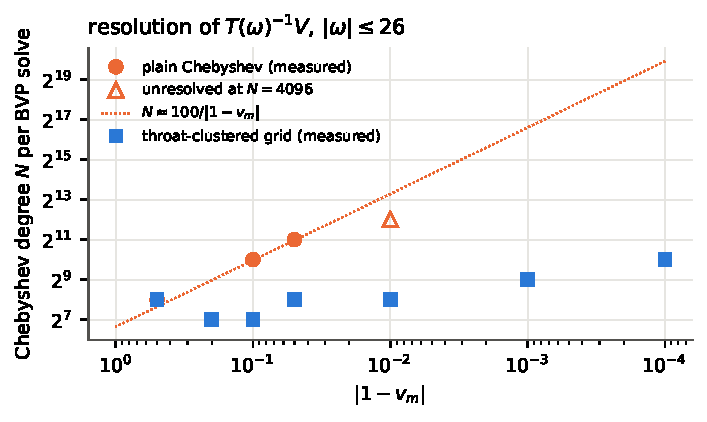
\includegraphics[width=0.62\textwidth]{resolution_vs_vm}
  \caption{Chebyshev degree reached by the adaptive BVP solver for $|\omega|\le26$, plain grid (orange) and
  throat-clustered grid (blue).}
  \label{fig:res}
\end{figure}

\begin{table}[H]\centering\footnotesize\begin{tabular}{llrrrrrr}
\toprule
$v_m$ & grid & scan [s] & BVP solves & max $N$ & \#eig & unpolished & unresolved tiles\\
\midrule
0.5 & plain (thesis run) & 9 & 3680 & 512 & 18 & 0 & 0\\
0.9 & plain & 376 & 4559 & 4096 & 25 & 5 & 0\\
\midrule
0.5 & mapped, $L=0.0$ & 9 & 3680 & 512 & 18 & 0 & 0\\
0.8 & mapped, $L=3.4$ & 4 & 2863 & 256 & 22 & 0 & 0\\
0.9 & mapped, $L=4.5$ & 7 & 5941 & 512 & 25 & 0 & 0\\
0.95 & mapped, $L=5.5$ & 23 & 11281 & 512 & 28 & 0 & 0\\
0.98 & mapped, $L=6.9$ & 37 & 12850 & 512 & 31 & 0 & 0\\
0.99 & mapped, $L=7.9$ & 87 & 16430 & 4096 & 33 & 1 & 0\\
1.5 & mapped, $L=0.0$ & 32 & 413 & 4096 & 7 & 1 & 0\\
1.3 & mapped, $L=0.0$ & 47 & 1921 & 4096 & 9 & 2 & 0\\
1.1 & mapped, $L=4.5$ & 4 & 2926 & 512 & 13 & 0 & 0\\
1.05 & mapped, $L=5.5$ & 8 & 2863 & 512 & 15 & 0 & 0\\
1.02 & mapped, $L=6.9$ & 13 & 3679 & 512 & 18 & 0 & 0\\
1.01 & mapped, $L=7.9$ & 54 & 5501 & 4096 & 21 & 1 & 0\\
1.005 & mapped, $L=8.9$ & 62 & 7637 & 4096 & 24 & 2 & 0\\
\bottomrule
\end{tabular}

  \caption{Full \infbeyn{} scans of the fixed-open window $\Real\omega\in[-0.5,26]$, $\Imag\omega\in[-3,3]$ on 12
  cores (4 for the second batch of mapped runs). ``max $N$'' is the degree of the longest eigenfunction.
  The plain-grid scan at $v_m=0.95$ is missing: it ran out of memory (see text).}
  \label{tab:timing}
\end{table}

\section{Is the Frobenius method good for the transonic flow?}

\paragraph{The idea, yes.} At $v_0=1$ the throat is a regular singular point of Eq.~\eqref{eq:nep}. Its
indicial exponents are $r=0$ (the regular solution) and
\begin{equation}
  r_s = -1 + \frac{i\omega}{v_0'(0)},\qquad \Real r_s = -1 - \frac{\Imag\omega}{v_0'(0)},\quad v_0'(0)=2.3238 .
\end{equation}
Requiring regularity is what turns the transonic problem into a well-posed eigenvalue problem, and it is the
correct physical condition. For $\Imag\omega<-v_0'(0)$ the second solution is also bounded, so ``regular'' must
then be read as ``analytic at the throat''. This is a modeling choice that the thesis makes implicitly.

\paragraph{The thesis implementation, no.} Three issues limit its accuracy:
\begin{enumerate}
  \item The recurrence linearizes $v_0$ and drops the $O(z)$ parts of the first- and zeroth-order
  coefficients. That leaves $c_0$ and $c_1$ exact but makes $c_2$ wrong by $O(1)$. For mode 1, the thesis
  value is $c_2=-0.82+0.51i$ and the exact one is $-1.32+0.05i$.
  \item The profile and its derivatives come from finite differences on 501 points and linear interpolation.
  The integration switches to the frozen series derivatives for $|z|<0.01$.
  \item The search is a Newton iteration from 11 starting points on the real axis. It is not exhaustive and
  can converge to non-eigenvalues of the discretized shooting function.
\end{enumerate}
Redoing the shooting carefully, with exact series coefficients started at $z=-10^{-3}$, an exact profile and
DOP853 at $10^{-10}$, moves the thesis eigenvalues by $9\times10^{-5}$ (mode 1), $0.07$ (mode 2) and
$1.5$--$4$ (modes 3--8). The last group no longer converges to the same points.

\paragraph{A better tool: \infbeyn{} with the regularity condition as a collocation row.} On the half nozzle
$[-1,0]$ (mapped to $[-1,1]$), the Chebyshev point at the throat is where $1-v_0^2=0$. Imposing the ODE
there, without a boundary condition, is exactly the Frobenius condition $c_1=-R_0c_0/Q_0$. The only boundary row
is $\tilde v(-1)=0$. Collocation picks the analytic solution automatically, and every solve resolves with
$N=64$. This is \texttt{TransonicInfBeyn} in \texttt{common.py}: it overrides the BVP matrix, the right-hand side
handling and the Newton derivative so that the throat row is treated as an equation, not a boundary row.
The scan of $\Real\omega\in[-0.5,22]$, $\Imag\omega\in[-6,3]$ takes about $110$\,s
(Fig.~\ref{fig:transonic}, Table~\ref{tab:transonic}). It finds exactly two eigenvalues above
$\Imag\omega\approx-5.4$:
\[
  \omega_1 = 3.687406-1.003933i,\qquad \omega_2 = 6.943383-3.181913i,
\]
both certified ($\gamma_{256}\sim10^{-9}$, halos $0.8$ and $0.03$), and both equal to the careful shooting
values to $10^{-5}$. The region where thesis modes 3--8 sit ($\Imag\omega\approx-3.8$) is resolved and contains
no eigenvalue. Below $\Imag\omega\approx-5.4$ the scan does not resolve, and $\gamma_n$ falls by an order of
magnitude for every unit of $\Imag\omega$, so the pseudospectrum fills that strip. The four careful-shooting
roots at $\Imag\omega\approx-5.4$ to $-5.5$ lie in it and cannot be certified.

\begin{figure}[H]
  \centering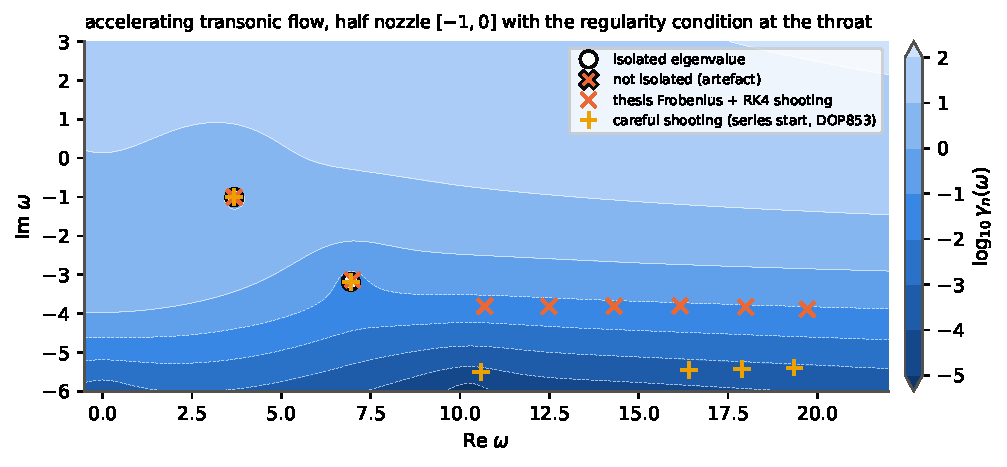
\includegraphics[width=\textwidth]{transonic_spectrum}\\
  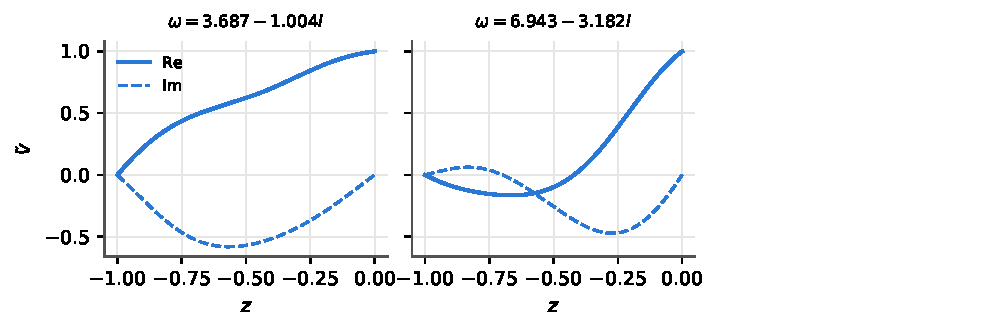
\includegraphics[width=\textwidth]{transonic_eigenfunctions}
  \caption{Accelerating transonic flow. Top: \infbeyn{} eigenvalues on the pseudospectrum, with the thesis
  shooting eigenvalues (orange crosses) and careful re-shooting from them (yellow plus signs). Bottom: the two
  eigenfunctions on the subsonic half; they are extended through the throat by the same regular solution.}
  \label{fig:transonic}
\end{figure}

\begin{table}[H]\centering\footnotesize\begin{tabular}{rlllll}
\toprule
$n$ & $\omega_n$ (InfBeyn) & $\gamma_{256}$ & halo & thesis shooting & $|\Delta|$\\
\midrule
1 & $3.687406-1.003933i$ & $2.2\times10^{-9}$ & $8.2\times10^{-1}$ & $3.6874-1.0040i$ & $8.8\times10^{-5}$\\
2 & $6.943383-3.181913i$ & $2.6\times10^{-9}$ & $3.2\times10^{-2}$ & $6.9954-3.1360i$ & $6.9\times10^{-2}$\\
\bottomrule
\end{tabular}

  \caption{Accelerating transonic flow: certified eigenvalues and the nearest thesis value.}
  \label{tab:transonic}
\end{table}

\paragraph{Verdict.} Use the Frobenius condition, but impose it inside \infbeyn{} rather than by shooting.
The transonic $v_m=1$ problem is then a first-class member of the same toolchain, at a cost comparable to a
non-transonic scan. One consequence matters for the transition study: the accelerating transonic flow is
damped in the window, with largest growth rate $\Imag\omega_1=-1.00$. The subsonic family stays weakly unstable
as $v_m\to1^-$ and the supersonic family strongly unstable as $v_m\to1^+$ (Sec.~\ref{sec:grid}). The transonic
spectrum is not the limit of either.

\section{How dense must the $v_m$ grid be?}\label{sec:grid}

\paragraph{Measurement.} Chebyshev collocation on the throat-clustered grid ($N=300$, keeping only eigenvalues
reproduced at $N=400$ to $10^{-6}$) is cheap enough to follow the whole window over 94 values of $v_m$ in
$[0.5,1.5]$. It took 21 minutes for fixed-open and 22 minutes for Dirichlet. It is used here only to measure
how the spectrum moves; the certified eigenvalues come from \infbeyn{}. Figure~\ref{fig:cont} shows the
spectra and, on the right, the median speed $|d\omega/dv_m|$ of the eigenvalues together with their minimum
spacing.

\begin{itemize}
  \item The spacing stays $O(1)$: $1.4\to0.5$ on the subsonic side, $3\to0.7$ on the supersonic side.
  \item The speed grows as $v_m\to1$: the median goes from $3$ at $v_m=0.5$ to $\sim200$ at $|1-v_m|=10^{-3}$,
  and the fastest mode is two to five times faster.
  \item Requiring that no eigenvalue moves more than a quarter of the spacing per step gives
  $\Delta v_m\approx0.11\,|1-v_m|$ on both sides. Examples: $0.011$ at $v_m=0.9$, $0.001$ at $0.99$,
  $0.0012$ at $1.01$, $0.013$ at $1.1$.
\end{itemize}

\paragraph{Recommendation.} Use a grid uniform in $\ln|1-v_m|$ with ratio $\approx0.9$ between consecutive
values of $|1-v_m|$, which is about 23 points per decade on each side:
\begin{center}
\begin{tabular}{lrr}
\toprule
range of $|1-v_m|$ & points per side & both sides\\
\midrule
$0.5\to10^{-2}$ & 40 & 80\\
$0.5\to10^{-3}$ & 62 & 124\\
$0.5\to10^{-4}$ & 85 & 170\\
\bottomrule
\end{tabular}
\end{center}
A grid uniform in $v_m$ would need $\Delta v_m\approx10^{-4}$ throughout, about $10^4$ points, to reach
$|1-v_m|=10^{-3}$. Tracking can be done by nearest neighbour between consecutive \infbeyn{} scans, or by
polishing the previous eigenvalues with \texttt{InfBeyn.polish}, with a full scan every few steps to catch modes
entering through the window edges.

\paragraph{Cost.} From Table~\ref{tab:timing}, a certified scan on the mapped grid costs $4$--$25$\,s for
$|1-v_m|\ge0.05$ and $50$--$90$\,s at $|1-v_m|=0.005$--$0.01$. The 80-point grid to $|1-v_m|=10^{-2}$ is about
$30$ minutes on this 12-core workstation. Below $10^{-2}$ the current implementation is limited by memory,
not by time:
\begin{itemize}
  \item \texttt{scan()} keeps every resolvent solve $T(z)^{-1}V$ (24 columns of Chebyshev coefficients) in a
  dictionary until the scan ends. At $v_m=0.995$ the parent process reached $10$\,GB after $10$ minutes and
  had to be stopped. Only the edge integrals and the node norms are needed once an edge is processed, so
  discarding the solutions after \texttt{\_segment\_integrals} would remove this.
  \item When \texttt{polish} does not converge it doubles $N$ up to \texttt{n\_max}$=4096$ in every worker. With
  12 workers this also exhausted the $15$\,GB. Use 4--6 workers or a lower \texttt{n\_max} near $v_m=1$.
\end{itemize}
With the cache fix, a rough extrapolation of Table~\ref{tab:timing} (solves growing like $|1-v_m|^{-0.4}$) puts
the 124-point grid to $10^{-3}$ at one to two hours. On the plain grid it is not feasible (Sec.~2).

\begin{figure}[H]\centering
  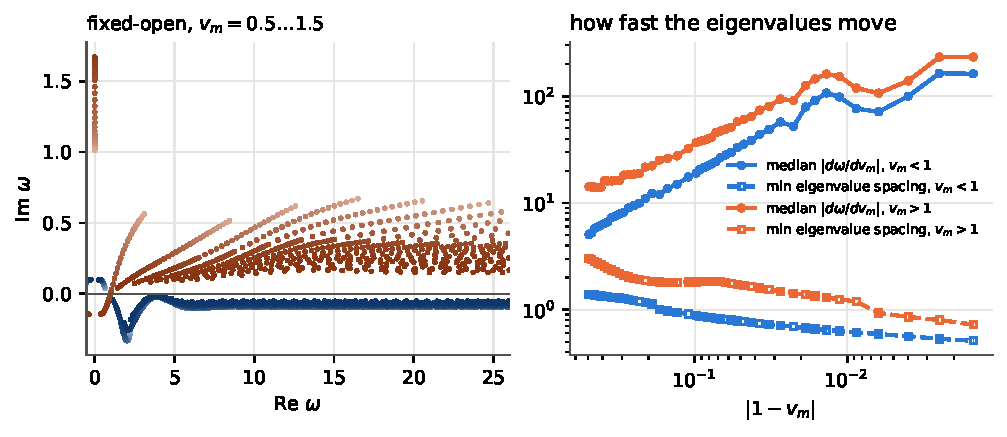
\includegraphics[width=\textwidth]{continuation_fixed_open}\\
  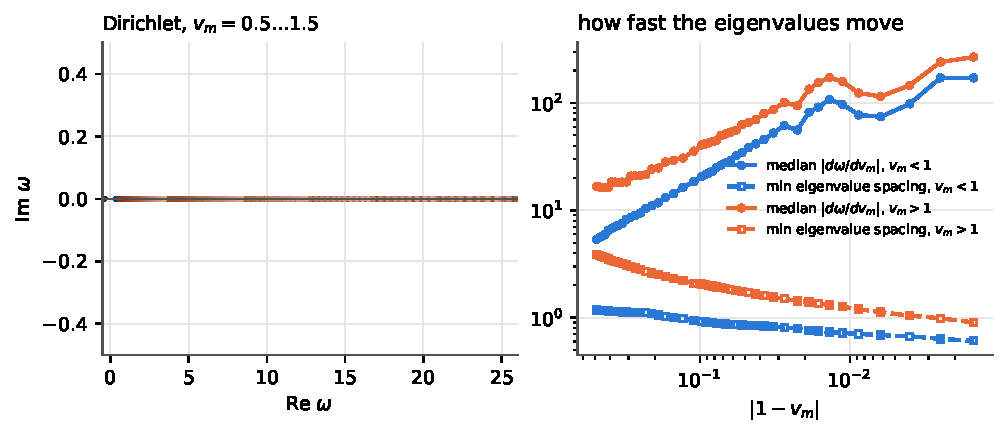
\includegraphics[width=\textwidth]{continuation_fixed_fixed}
  \caption{Collocation continuation in $v_m$ (fixed-open top, Dirichlet bottom). Left: all converged
  eigenvalues for $v_m=0.5\ldots0.999$ (blue, darker closer to 1) and $1.001\ldots1.5$ (orange). Right: median
  eigenvalue speed and minimum spacing against $|1-v_m|$.}
  \label{fig:cont}
\end{figure}

\paragraph{First look at the transition (fixed-open).} The largest growth rate on the subsonic side rises
slowly, from $0.039$ at $v_m=0.5$ to about $0.10$ at $v_m=0.99$ (the unstable ground mode). On the supersonic
side it rises from $1.01$ at $v_m=1.5$ to $1.67$ just above $v_m=1$ (the purely imaginary mode). The jump in
growth rate across $v_m=1$ is therefore a factor of about 16. The subsonic spectrum gets denser as $v_m\to1^-$,
with 18 eigenvalues in the window at $0.5$ and 39 at $0.998$. With Dirichlet boundaries all eigenvalues stay
real on both sides. Figures~\ref{fig:sweep} and \ref{fig:growth} show the certified \infbeyn{} spectra from the
sweep.

\begin{figure}[H]\centering
  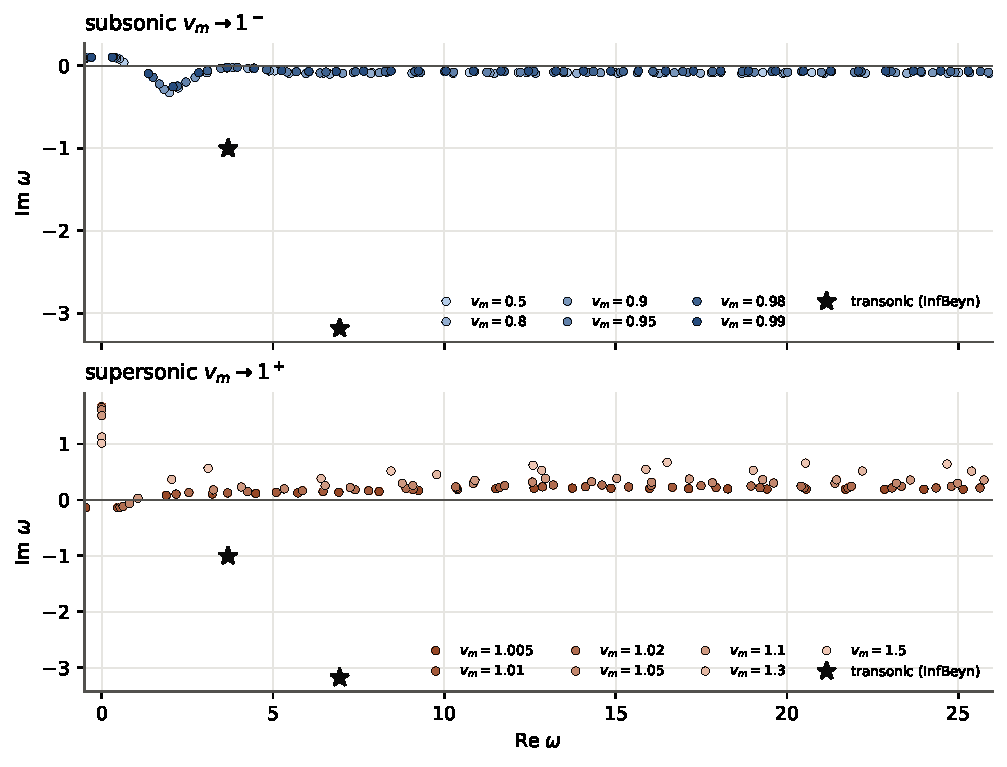
\includegraphics[width=\textwidth]{sweep_spectra}
  \caption{Certified \infbeyn{} spectra (fixed-open) at the swept $v_m$ (darker closer to $1$), with the
  transonic eigenvalues (stars).}
  \label{fig:sweep}
\end{figure}
\begin{figure}[H]\centering
  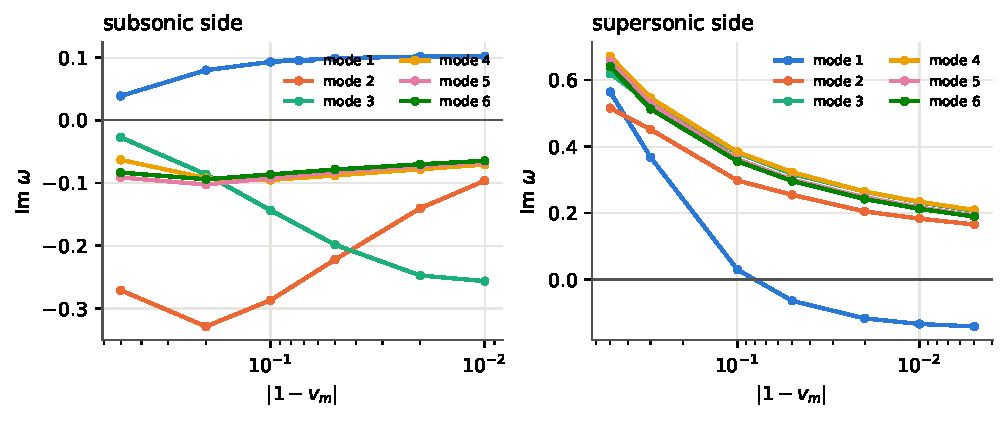
\includegraphics[width=\textwidth]{sweep_growth_rates}
  \caption{Growth rates of the six lowest modes with $\Real\omega>0.05$ along the \infbeyn{} sweep, tracked by
  nearest neighbour. The sweep is much coarser than the recommended grid (steps of $0.2$ between $v_m=1.5$, $1.3$,
  $1.1$, against $\Delta v_m\approx0.03$ needed there), so the mode labels may swap. The drop of supersonic
  mode 1 below zero is confirmed by the collocation continuation: it crosses between $v_m=1.080$ and $1.085$
  (Sec.~\ref{sec:neutral}). The purely imaginary supersonic mode ($\Real\omega=0$) is excluded here; its growth
  rate rises from $1.01$ to $1.67$.}
  \label{fig:growth}
\end{figure}

\paragraph{A mirrored pattern near the sonic point (fixed-open).}\label{sec:neutral} Since the spectrum is
symmetric under $\omega\mapsto-\bar\omega$, only $\Real\omega>0.05$ is considered here, and the purely imaginary
supersonic mode is set aside. Modes are numbered by increasing $\Real\omega$. Close to $v_m=1$ the two sides
are mirror images of each other:
\begin{itemize}
  \item Subsonic: the bulk of the spectrum is damped, mode 1 (the ground mode) is unstable
  ($\Imag\omega_1\approx+0.10$), and $\Imag\omega_2\to0^-$.
  \item Supersonic: the bulk of the spectrum grows, mode 1 is stable ($\Imag\omega_1\approx-0.14$), and
  $\Imag\omega_2\to0^+$.
\end{itemize}
Mode 2 looks as if it is about to cross the real axis, but down to $|1-v_m|=10^{-3}$ it has not crossed on
either side. Its growth rate decreases like a power of $|1-v_m|$ (Table~\ref{tab:neutral}); least-squares fits of
$\ln|\Imag\omega_2|$ against $\ln|1-v_m|$ over $|1-v_m|\le0.02$ give
\begin{equation}
  \Imag\omega_2\approx-1.12\,(1-v_m)^{0.53}\quad(v_m\to1^-),\qquad
  \Imag\omega_2\approx+0.56\,(v_m-1)^{0.37}\quad(v_m\to1^+).
\end{equation}
The subsonic side is close to a $\sqrt{1-v_m}$ law ($\Imag\omega_2/\sqrt{1-v_m}$ stays between $-0.99$ and
$-0.92$). On the supersonic side the same ratio grows from $0.92$ to $1.31$, so the approach is slower than a
square root. Extrapolated, both fits reach $\Imag\omega_2=0$ exactly at $v_m=1$: mode 2 becomes neutral in the
limit, from below on the subsonic side and from above on the supersonic side. This is an extrapolation from
$|1-v_m|\ge10^{-3}$ (the continuation at $v_m=0.999$ did not converge for mode 2 and is left out). A log-log fit on
the fine grid of Sec.~\ref{sec:grid}, and a check of whether mode 3 behaves the same way closer to $v_m=1$, would
show whether $v_m=1$ is a single neutral point or an accumulation of them.

\begin{table}[H]\centering\footnotesize
\begin{tabular}{lrrr@{\qquad}lrrr}
\toprule
$v_m$ & $\Imag\omega_1$ & $\Imag\omega_2$ & $\Imag\omega_2/\sqrt{1-v_m}$ &
$v_m$ & $\Imag\omega_1$ & $\Imag\omega_2$ & $\Imag\omega_2/\sqrt{v_m-1}$\\
\midrule
$0.980$ & $0.102$ & $-0.140$ & $-0.99$ & $1.020$ & $-0.117$ & $0.130$ & $0.92$\\
$0.985$ & $0.102$ & $-0.120$ & $-0.98$ & $1.010$ & $-0.133$ & $0.102$ & $1.02$\\
$0.990$ & $0.102$ & $-0.096$ & $-0.96$ & $1.0075$ & $-0.137$ & $0.092$ & $1.07$\\
$0.9925$ & $0.102$ & $-0.082$ & $-0.95$ & $1.005$ & $-0.141$ & $0.080$ & $1.13$\\
$0.995$ & $0.101$ & $-0.067$ & $-0.94$ & $1.003$ & $-0.143$ & $0.066$ & $1.20$\\
$0.997$ & $0.101$ & $-0.051$ & $-0.93$ & $1.002$ & $-0.144$ & $0.056$ & $1.26$\\
$0.998$ & $0.100$ & $-0.041$ & $-0.92$ & $1.001$ & $-0.144$ & $0.042$ & $1.31$\\
\bottomrule
\end{tabular}
\caption{Growth rates of the two lowest modes with $\Real\omega>0.05$ near the sonic point, from the collocation
continuation (throat-clustered grid, $N=300$, reproduced at $N=400$ to $10^{-6}$). They agree with the certified
\infbeyn{} sweep at $v_m=0.99$, $1.005$, $1.01$, $1.02$.}
\label{tab:neutral}
\end{table}

Away from $v_m=1$ the mirror breaks. The subsonic ground mode is unstable for every $v_m$ checked, down to
$v_m=0.05$ ($\Imag\omega_1=0.0025$, roughly $0.05\,v_m$ for small $v_m$; plain-grid collocation, $N=300$
against $400$). The constant-profile limit has every mode damped, so the profile variation itself destabilizes
the ground mode. The stable supersonic mode 1 instead exists only in a thin layer: $\Imag\omega_1$ crosses zero
between $v_m=1.080$ ($-0.008$) and $1.085$ ($+0.001$), and for larger $v_m$ (checked up to $3$) every mode with
$\Real\omega>0$ is unstable. The purely imaginary supersonic mode also has no subsonic counterpart: for constant
$v_0$ the subsonic real parts are shifted by half a spacing, so no subsonic eigenvalue sits on the imaginary axis.

\section{Summary}
\begin{itemize}
  \item \textbf{\infbeyn{}} is ready for $v_m\ne1$ once the grid is clustered at the throat. That change is
  in \texttt{common.py} (\texttt{mapped\_problem}); without it the method fails below $|1-v_m|\approx0.05$.
  \item \textbf{Frobenius}: the regularity condition is the right physics. Imposed as a collocation row inside
  \infbeyn{} it gives certified transonic eigenvalues. The thesis shooting results are correct only for the first
  mode, and modes 3--8 are not eigenvalues.
  \item \textbf{Grid}: logarithmic in $|1-v_m|$, about 23 points per decade per side. That is 80 scans to reach
  $|1-v_m|=10^{-2}$ (about 30 minutes now) or 124 to reach $10^{-3}$ (one to two hours, after the solution-cache
  memory fix in \texttt{scan()}).
  \item \textbf{Open point}: the limits $v_m\to1^\pm$ approach cusped profiles, and their spectra differ from
  the accelerating transonic spectrum. Deciding which object ``the spectrum at the sonic point'' should be
  is a physics question to settle before running the full sweep.
\end{itemize}

\paragraph{Files.} \texttt{common.py} contains the profiles, the mapped problem, \texttt{TransonicInfBeyn} and
collocation. \texttt{scan\_sweep.py} runs the mapped \infbeyn{} sweep, \texttt{scan\_timing.py} the plain-grid
timing, \texttt{transonic\_scan.py} the transonic problem, \texttt{frobenius\_check.py} the series and
re-shooting check, and \texttt{continuation.py} the collocation continuation. \texttt{make\_figures.py}
produces all figures and tables.

\begin{thebibliography}{9}
\bibitem{feng2024} H.~Feng, \emph{Spectral stability of plasma flows in the magnetic nozzle}, M.Sc.\ thesis,
University of Saskatchewan, 2024.
\bibitem{colbrook2023} M.~J.~Colbrook and A.~Townsend, \emph{Avoiding discretization issues for nonlinear
eigenvalue problems}, arXiv:2305.01691, 2023.
\end{thebibliography}
\end{document}
